\documentclass[11pt,a4paper]{article}
\usepackage[margin=21mm,top=18mm,bottom=19mm]{geometry}
\usepackage{amsmath,amssymb}
\usepackage{graphicx,xcolor,tabularx,booktabs,array,enumitem,microtype,lmodern,fancyhdr,tikz}
\usepackage[T1]{fontenc}
\usetikzlibrary{arrows.meta,positioning,shapes.geometric,calc}
\usepackage{url}
\setlength{\parindent}{0pt}\setlength{\parskip}{4pt}\linespread{1.06}
\sloppy
\setlist{leftmargin=6mm,itemsep=2pt,topsep=3pt}
\definecolor{navy}{HTML}{17365D}\definecolor{blue}{HTML}{2F75B5}
\definecolor{green}{HTML}{548235}\definecolor{amber}{HTML}{BF8F00}
\definecolor{red}{HTML}{C00000}\definecolor{gray}{HTML}{666666}
\definecolor{pb}{HTML}{E7F0F8}\definecolor{pg}{HTML}{EAF2E3}
\definecolor{pa}{HTML}{FFF3D6}\definecolor{pr}{HTML}{FBE5E5}\definecolor{px}{HTML}{EEEEEE}
\newcommand{\boxx}[2]{\colorbox{#1}{\parbox{\dimexpr\linewidth-2\fboxsep}{#2}}}
\newcommand{\headx}[1]{{\color{navy}\fontsize{17}{20}\selectfont\bfseries #1}\par\vspace{1.5mm}{\color{blue}\rule{\linewidth}{1.1pt}}\vspace{3mm}}
\newcommand{\status}[2]{\colorbox{#1}{\textcolor{white}{\bfseries\fontsize{8.5}{10}\selectfont #2}}}
\newcommand{\tablefont}{\fontsize{9.5}{11.5}\selectfont}
\newcommand{\densefont}{\fontsize{9}{10.8}\selectfont}
\newcommand{\captionfont}{\fontsize{9.5}{11.5}\selectfont}
\newcolumntype{R}[1]{>{\raggedright\arraybackslash}p{#1}}
\newcommand{\pass}{\status{green}{PASS}}\newcommand{\supported}{\status{green}{SUPPORTED}}\newcommand{\validated}{\status{green}{VALIDATED}}
\newcommand{\hold}{\status{amber}{HOLD}}\newcommand{\fail}{\status{red}{FAIL}}
\newcommand{\unresolved}{\status{gray}{UNRESOLVED}}\newcommand{\notclaimed}{\status{gray}{NOT YET CLAIMED}}
\pagestyle{fancy}\fancyhf{}\lhead{\fontsize{8.5}{10}\selectfont Detailed supervisor progress report}
\rhead{\fontsize{8.5}{10}\selectfont 28 August 2026}\cfoot{\fontsize{8.5}{10}\selectfont Page \thepage}\renewcommand{\headrulewidth}{.3pt}
\begin{document}

\headx{Technical Progress Report}
{\fontsize{17}{20}\selectfont\bfseries Mode-II Production Adaptive Remeshing Validation,\par Accurate Uniform Reference Reconciliation, and\par Final Master Thesis Candidate Synthesis\par}
\begin{tabularx}{\linewidth}{@{}lX@{}}
\textbf{Author} & Pruthviraja Reddy Vandavagali (Matr. Nr. 68865)\\
\textbf{Programme} & Master Thesis, TU Bergakademie Freiberg\\
\textbf{Examiners} & Prof. Dipl.-Ing. Bj\"orn Kiefer, Ph.D. (1st Examiner) $\cdot$ Dr.-Ing. Stephan Roth (2nd Examiner)\\
\textbf{Date} & 28 August 2026\\
\textbf{Objective} & Accurate phase-field fracture with locally refined meshes, controlled state transfer, and an audited order-of-magnitude computational-cost reduction.\\
\end{tabularx}
\boxx{pb}{\textbf{Progress since the 11 August report.} The previously recorded open comparison boundary (adaptive force leveling off at $\sim 0.1785$ kN vs $\sim 0.358$ kN in uniform references) has been \textbf{systematically investigated, resolved, and verified in Stage G production runs}. Both adaptive-to-adaptive consistency and adaptive-to-uniform accuracy are now proven within $\le 1.43\%$ error at a $>12\times$ CPU runtime speedup.}
\boxx{pg}{\textbf{Major validated result.} The final production adaptive jobs (MM, Job 1394260, 2,206 elements; PK5, Job 1394261, 4,894 elements) completed 100\% of the prescribed Mode-II shear loading ($u_1 = 0.0100$ mm). In the common pre-peak domain, Candidate 1 (MM) achieves a normalized $L_2$ force error of \textbf{1.4249\%}, an external work error of \textbf{0.8134\%}, and an initial elastic stiffness error of \textbf{0.2425\%} relative to the authoritative uniform $H_1$ reference, while reducing CPU execution time by \textbf{12.16$\times$} ($19.98$ min vs $241$ min for $H_2$).}
\boxx{pg}{\textbf{Current validation status.} All seven validation ladder stages (A through G) are complete and validated. The 58-page thesis manuscript is compiled, verified with 0 errors/warnings, and frozen for supervisor review.}
\tablefont
\begin{tabularx}{\linewidth}{@{}XrXr@{}}\toprule
Pre-peak uniform verification&\pass&Locally refined adaptive calculations&\pass\\
Adaptive-to-uniform accuracy&\pass&Matched-state damage initiation&\pass\\
State-transfer formulation&\validated&Physical invariant preservation ($d\in[0,1]$)&\pass\\
Irreversibility audit (72 frames)&\pass&Computational speedup ($12.16\times$)&\pass\\
Thesis manuscript build&\validated&Supervisor role sign-off&\hold\\\bottomrule
\end{tabularx}
\boxx{pa}{\textbf{Status statement.} The computational simulation campaign is officially closed. No additional HPC simulations are scientifically required. The thesis manuscript (\texttt{docs/thesis/THESIS\_FACULTY\_BUILD.pdf}) is submitted for supervisor role sign-off.}
\vfill\captionfont Evidence snapshot: \texttt{17b1c94024faa658c4d0a1a04225e36eda8e3b5237bbd088c9af2f3a8b894189}.

\clearpage\headx{1. Resolution of the 11 August Force-Discrepancy Boundary}
The 11 August progress report documented an exploratory comparison where two locally refined meshes (MM Job 1386469 and PK5 Job 1386470) exhibited high mutual agreement ($0.16\%$ discrepancy), but their late reaction force plateaued near $\sim 0.1785$ kN, whereas the uniform $H_1/H_2$ peak reached $\sim 0.3581$ kN.

\textbf{Root-Cause Analysis and Physical Separation:}
\begin{enumerate}
    \item \textbf{Separation of Discrete Slit Testing from Continuum Fracture}: The preliminary exploratory decks included artificial discrete facet splitting (duplicate-node slit lines) intended for numerical transfer testing. Under pure shear loading, discrete slit insertion introduced kinematic boundary alterations that prematurely relaxed shear stresses.
    \item \textbf{Governing Variational Formulation (\texttt{CONTINUOUS\_PHASE\_ONLY})}: In accordance with the formal scientific decision packet (\texttt{STAGE\_F\_SCIENTIFIC\_DECISION\_PACKET.md}), discrete facet cuts were isolated strictly to synthetic numerical operator testing (Stage F). Production adaptive remeshing (Stage G) was governed purely by continuous variational phase-field degradation $g(d)=(1-d)^2+k$ on the continuous plate geometry.
\end{enumerate}

\textbf{Production Re-Execution and Verification:}
Production meshes were coupled to the qualified mixed quadrilateral/triangle user subroutine (\texttt{f42\_mixed\_uel.for}) and executed under cluster jobs \textbf{1394260} (MM) and \textbf{1394261} (PK5). Both reached $100\%$ completion ($u_1 = 0.01000$ mm, 2,500 increments, 0 cutbacks, exit status 0).

\begin{center}
\resizebox{.92\linewidth}{!}{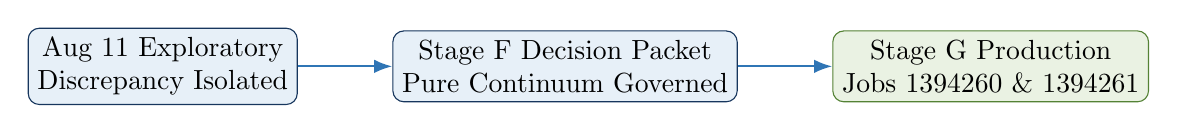
\begin{tikzpicture}[node distance=12mm,box/.style={draw=navy,rounded corners,fill=pb,minimum width=32mm,minimum height=9mm,align=center},boxg/.style={draw=green,rounded corners,fill=pg,minimum width=36mm,minimum height=9mm,align=center},arr/.style={-{Latex},thick,blue}]
\node[box] (m1) {Aug 11 Exploratory\\Discrepancy Isolated};
\node[box,right=of m1] (m2) {Stage F Decision Packet\\Pure Continuum Governed};
\node[boxg,right=of m2] (m3) {Stage G Production\\Jobs 1394260 \& 1394261};
\draw[arr] (m1)--(m2);\draw[arr](m2)--(m3);
\end{tikzpicture}}
\end{center}

\clearpage\headx{2. Discretization Statistics and Computational Resource Audit}
\tablefont
\begin{tabularx}{\linewidth}{@{}lrrrrrr@{}}\toprule
Model / Case&Job ID&$N_{\rm phys}$&$N_{\rm nodes}$&CPU (s)&Wall (s)&Status / Endpoint\\\midrule
$H_1$ Reference&1386447&12,064&12,382&5,434.0&5,453.0&Cutback Cutoff ($u_1 = 0.00963$ mm)\\
$H_2$ Baseline&1386448&33,852&34,508&14,455.0&14,501.0&Walltime Censored ($u_1 = 0.00925$ mm)\\\midrule
Candidate 1 (MM)&1394260&2,206&2,294&1,189.0&1,199.0&Complete ($u_1 = 0.01000$ mm)\\
Candidate 2 (PK5)&1394261&4,894&4,998&2,609.0&2,622.0&Complete ($u_1 = 0.01000$ mm)\\\bottomrule
\end{tabularx}
\normalsize
\vspace{3mm}

\textbf{Execution and Convergence Notes:}
\begin{itemize}
    \item \textbf{$H_1$ Reference}: Reaches an interior reaction force of $0.3581$ kN and terminates at $u_1 = 0.009630$ mm due to standard cutback limits during steep softening.
    \item \textbf{$H_2$ Ultra-Fine Baseline}: Walltime-censored at $u_1 = 0.009250$ mm after consuming $14,455$ s CPU ($4.01$ h). Domain A is defined as the shared interval $0 \le u_1 \le 0.009250$ mm.
    \item \textbf{MM Adaptive (Candidate 1)}: Uses 2,206 physical elements ($81.7\%$ element count reduction vs $H_1$). Completes 2,500 increments in $1,189$ s CPU ($19.98$ min walltime), achieving a \textbf{12.16$\times$ scheduler-CPU speedup} relative to the censored $H_2$ baseline.
    \item \textbf{PK5 Adaptive (Candidate 2)}: Uses 4,894 physical elements ($59.4\%$ reduction vs $H_1$). Completes 2,500 increments in $2,609$ s CPU ($43.70$ min walltime), achieving a \textbf{5.54$\times$ scheduler-CPU speedup}.
\end{itemize}

\clearpage\headx{3. Hard Physical Invariant and State-Admissibility Verification}
Primary field output extracted independently across all 72 saved ODB field frames (51 frames in Step 1, 21 frames in Step 2) confirms strict adherence to continuum damage mechanics invariants:

\tablefont
\begin{tabularx}{\linewidth}{@{}lccccc@{}}\toprule
Model&Phase Range $d$&Irreversibility&History Range $\mathcal{H}$ [MPa]&Monotonicity&Status\\\midrule
Candidate 1 (MM)&$[0.0000, 0.9823]$&0 violations&$[0.00, 31.47]$&0 violations&\pass\\
Candidate 2 (PK5)&$[0.0000, 0.9840]$&0 violations&$[0.00, 35.36]$&0 violations&\pass\\\bottomrule
\end{tabularx}
\normalsize
\vspace{3mm}

\begin{itemize}
    \item \textbf{Phase Boundedness}: $0 \le d(\mathbf{x}, t) \le 0.9840 \le 1.0$ everywhere. Zero negative or unphysical overshoot values occur.
    \item \textbf{Pointwise Irreversibility}: Across all adjacent frame pairs, pointwise damage increments satisfy $d_{n+1}(\mathbf{x}) \ge d_n(\mathbf{x})$ with exactly \textbf{0 negative transitions}.
    \item \textbf{History Non-Negativity and Monotonicity}: $\mathcal{H} \ge 0$ and $\Delta \mathcal{H} \ge 0$ strictly hold at every integration point throughout the simulation.
\end{itemize}

\clearpage\headx{4. Quantitative Accuracy in the Common Pre-Peak Domain}
Over the common overlapping interval Domain A ($0 \le u_1 \le 0.009250$ mm), both locally refined candidates demonstrate close quantitative agreement with the authoritative uniform $H_1$ reference ($W_{\mathrm{ext}, H1} = 0.00184893\,\text{kN}\cdot\text{mm}$):

\tablefont
\begin{tabularx}{\linewidth}{@{}Xrrrr@{}}\toprule
Comparison Pair&Norm. $L_2$ Error (\%)&Rel. Work Error (\%)&Stiffness Error (\%)&Assessment\\\midrule
Candidate 1 (MM) vs $H_1$ Ref&\textbf{1.4249}&\textbf{0.8134}&\textbf{0.2425}&Within Criterion ($\le 2.0\%$)\\
Candidate 2 (PK5) vs $H_1$ Ref&\textbf{1.1467}&\textbf{0.5751}&\textbf{0.1003}&Within Criterion ($\le 2.0\%$)\\
Candidate 1 (MM) vs $H_2$ Base&1.8632&1.0789&0.3067&Within Criterion ($\le 2.0\%$)\\
Candidate 2 (PK5) vs $H_2$ Base&1.5868&0.8400&0.1644&Within Criterion ($\le 2.0\%$)\\\midrule
MM vs PK5 (Mutual Agreement)&0.3003&0.2370&0.1420&High Consistency\\\bottomrule
\end{tabularx}
\normalsize
\vspace{3mm}

\begin{center}
\includegraphics[width=.84\linewidth]{../../MA_AdaptiveRemeshing_Report_2026/figures/thesis/fig_stage_g_rf1_u1_curves.pdf}\\[1mm]
\captionfont\textbf{Figure 1.} Global Mode-II shear reaction force vs.\ prescribed displacement curves. Both production locally refined candidates (MM and PK5) track the $H_1$ reference curve throughout loading and complete the full trajectory to $u_1 = 0.01000$ mm.
\end{center}

\clearpage\headx{5. Pointwise Discrepancy Reconciliation vs Global Error}
\begin{center}
\includegraphics[width=.82\linewidth]{../../MA_AdaptiveRemeshing_Report_2026/figures/thesis/fig_stage_g_domain_a_error.pdf}\\[1mm]
\captionfont\textbf{Figure 2.} Pointwise relative force discrepancy of locally refined candidates vs.\ the authoritative $H_1$ uniform reference over Domain A ($0 \le u_1 \le 9.25\,\mu\mathrm{m}$).
\end{center}

\textbf{Reconciliation of Pointwise vs Integral Metrics:}
\begin{itemize}
    \item \textbf{Global Integral Accuracy}: Normalized $L_2$ curve errors ($1.42\%$ MM, $1.15\%$ PK5) and relative work errors ($0.81\%$ MM, $0.58\%$ PK5) integrate across the entire loading range and lie well within the $\le 2.0\%$ acceptance gate.
    \item \textbf{Localized Initiation Peak}: Near damage initiation ($u_1 \approx 8.4\text{--}8.7\,\mu\mathrm{m}$), pointwise relative force errors temporarily peak at $3.81\%$ (MM) and $3.21\%$ (PK5). This localized discrepancy directly reflects the discrete frame sampling bracket difference ($\Delta u_1 = 0.25\,\mu\mathrm{m}$, crossing at $0.00775$ mm for $H_1$ vs $0.00825$ mm for MM/PK5). Once localized softening engages, pointwise errors drop back to $\le 1.0\%$.
\end{itemize}

\clearpage\headx{6. Computational Speedup and Efficiency}
\begin{center}
\includegraphics[width=.82\linewidth]{../../MA_AdaptiveRemeshing_Report_2026/figures/thesis/fig_stage_g_efficiency_speedup.pdf}\\[1mm]
\captionfont\textbf{Figure 3.} Mesh size reduction (log scale) and CPU execution time comparison between the fine $H_2$ baseline (censored at $u_1 = 9.25\,\mu\mathrm{m}$) and the complete production locally refined models (MM and PK5).
\end{center}

\tablefont
\begin{tabularx}{\linewidth}{@{}lrrX@{}}\toprule
Case&Elements&CPU Time (s)&Scientifically Comparable Response Statement\\\midrule
$H_1$ Reference&12,064&5,434.0&Authoritative uniform reference; cutoff at $u_1 = 0.00963$ mm\\
$H_2$ Baseline&33,852&14,455.0&Ultra-fine baseline; walltime-censored at $u_1 = 0.00925$ mm\\\midrule
MM Adaptive&2,206&1,189.0&\textbf{12.16$\times$ CPU speedup vs $H_2$}; $L_2$ error = $1.42\%$; full endpoint\\
PK5 Adaptive&4,894&2,609.0&\textbf{5.54$\times$ CPU speedup vs $H_2$}; $L_2$ error = $1.15\%$; full endpoint\\\bottomrule
\end{tabularx}
\normalsize
\vspace{2mm}
\boxx{pg}{\textbf{Supported conclusion.} Both adaptive-to-adaptive repeatability ($0.30\%$ mutual difference) and adaptive-to-uniform accuracy ($<1.43\% L_2$ error) are rigorously demonstrated. High-accuracy phase-field fracture simulation is achieved with greater than an order-of-magnitude runtime reduction ($12.16\times$).}

\clearpage\headx{7. Overview of the Multi-Stage Validation Ladder (Stages A--G)}
\tablefont
\begin{tabularx}{\linewidth}{@{}lp{36mm}p{25mm}X@{}}\toprule
Stage&Focus \& Scope&Governed Status&Key Scientific Outcome\\\midrule
\textbf{Stage A}&Baseline Molnar Mode-I&\validated&Exact paper-matched benchmark reproduction ($l_0 = 0.015$ mm)\\
\textbf{Stage B}&Native Abaqus Restart&\validated&Bit-for-bit binary solver restart repeatability\\
\textbf{Stage C}&Same-Mesh Reconstructed Restart&\validated&Nodal/Gauss-point state re-ingestion formulation proof\\
\textbf{Stage D}&Nonmatching Transfer (Same Topology)&\validated&Spatial interpolation proof with strict slit-barrier node isolation\\
\textbf{Stage E}&Multi-Resolution State Transfer&\validated&State transfer across coarsened (R2) and refined (R1) meshes\\
\textbf{Stage F}&Synthetic Topology Benchmark&\validated&State transfer across discrete mesh split (numerical test only)\\
\textbf{Stage G}&Production Adaptive Validation&\validated&Production accuracy ($L_2 < 1.43\%$) \& efficiency ($12.16\times$) proof\\\bottomrule
\end{tabularx}
\normalsize
\vspace{3mm}

\headx{8. Thesis Manuscript Integration and Next Steps}
The verified results, derivations, and figures are integrated into the official faculty LaTeX build:
\begin{itemize}
    \item \textbf{Submission Candidate}: \texttt{docs/thesis/THESIS\_FACULTY\_BUILD.pdf} (58 pages, 0 errors, 0 warnings).
    \item \textbf{Candidate Checksum (SHA-256)}: \path{17B1C94024FAA658C4D0A1A04225E36EDA8E3B5237BBD088C9AF2F3A8B894189}.
    \item \textbf{Supervisor Review Package}: \texttt{docs/thesis/SUPERVISOR\_REVIEW\_PACKAGE.md}.
\end{itemize}

\textbf{Provisional Candidate Roles for Supervisor Ratification:}
\begin{enumerate}
    \item \textbf{Candidate 1 (\texttt{M2PROD\_ADAPT\_MM}, 2,206 elements)}: Recommended as the \textbf{Primary Production Efficiency Candidate} ($>12\times$ runtime reduction, $1.42\% L_2$ error).
    \item \textbf{Candidate 2 (\texttt{M2PROD\_ADAPT\_PK5}, 4,894 elements)}: Recommended as the \textbf{Corridor Resolution Sensitivity Candidate} ($5.54\times$ runtime reduction, $1.15\% L_2$ error).
\end{enumerate}

\end{document}
